\documentclass[a4paper]{article}

%% Language and font encodings
\usepackage[english]{babel}
\usepackage[utf8x]{inputenc}
\usepackage[T1]{fontenc}
\usepackage[section]{placeins}
\usepackage{graphicx}
\usepackage{caption}
\usepackage{subcaption}

\usepackage{fancyvrb}	

%\usepackage{pdfpages}%to insert pdfs
 
\usepackage{float}		%Ben trying to format figures

%% Sets page size and margins
\usepackage[a4paper,top=3cm,bottom=2cm,left=3cm,right=3cm,marginparwidth=1.75cm]{geometry}

%% Useful packages
\usepackage{amsmath}
\usepackage{graphicx}
\usepackage[colorinlistoftodos]{todonotes}
\usepackage[colorlinks=true, allcolors=blue]{hyperref}
\makeatletter

%% All below Added by Ben |||||||||||||||||||||||||||||||||||||||||||||||
\g@addto@macro\@floatboxreset\centering
\makeatother				% this and above automatically center figures

% Alphabetized list macro from:  https://tex.stackexchange.com/questions/121489/alphabetically-display-the-items-in-itemize
\usepackage{datatool}% http://ctan.org/pkg/datatool
\newcommand{\sortitem}[1]{%
  \DTLnewrow{list}% Create a new entry
  \DTLnewdbentry{list}{description}{#1}% Add entry as description
}
\newenvironment{sortedlist}{%
  \DTLifdbexists{list}{\DTLcleardb{list}}{\DTLnewdb{list}}% Create new/discard old list
}{%
  \DTLsort{description}{list}% Sort list
  \begin{itemize}%
    \DTLforeach*{list}{\theDesc=description}{%
      \item \theDesc}% Print each item
  \end{itemize}%
}
%use these instead to alphabetize list:
%\begin{sortedlist}
%   \sortitem{ISDYNSTP
%
%||||||||||||||||||||||||||||||||||||||||||||||||||||||||||||||||||||||||||


\title{ECE271, Final Project}
\author{Ben Adams, Grant Haines, Benjiman Walsh}
\date{\today}

\begin{document}
\maketitle

\pagebreak

\tableofcontents

\section{Introduction}

The purpose of this project is to create a digital logic design that uses various parallel input modules with various output modules for implementation on an Field Programmable Gate Array- or FPGA. FPGA programming and design allows smaller digital logic modules to be implemented all on the same board. This paper discusses a number of input and output modules and an easily implementable top-level example design that ties all of these modules together. 


\section{High Level Descriptions}%%%%%%%%%%%%%%


\section{Controller Descriptions}

This section is meant to provide a brief but thorough low-level view of the operations of our chosen input devices. 

\subsection{NES Controller}

The Nintendo Entertainment System (NES) first became available in America in 1985 and revolutionized society as the first accessible home video game system. NES controllers (pictured in figure \ref{nesController}) work by receiving "clock" and "latch" signals from the NES console and transmitting a data signal to the console. NES controllers use a shift register to store all of the controller's button data when the console sends the latch signal (As in figure \ref{nesSchematic}). Each successive clock signal shifts the controller register down and the controller's data wire outputs a value that represents the next button's signal (See figure \ref{nesClock}). 

\begin{figure}[H]
    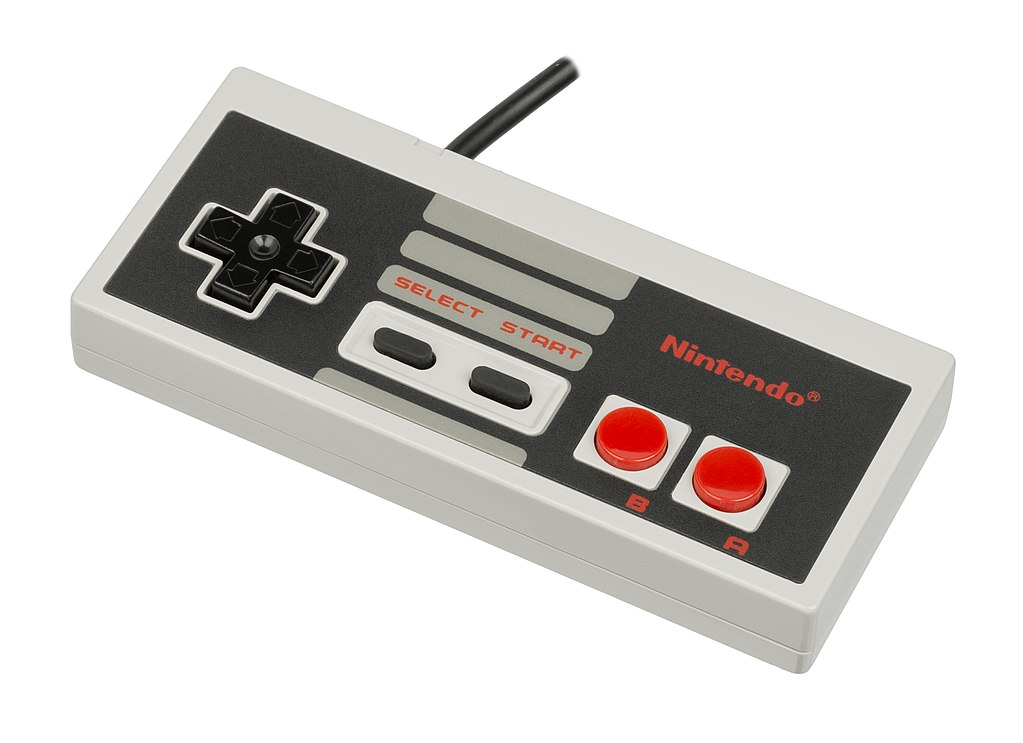
\includegraphics[width=0.6 \linewidth]{images/NEScontroller.jpg}
    \caption{An NES controller (Picture courtesy of Wikipedia)}
    \label{nesController}
\end{figure}

\begin{figure}[H]
    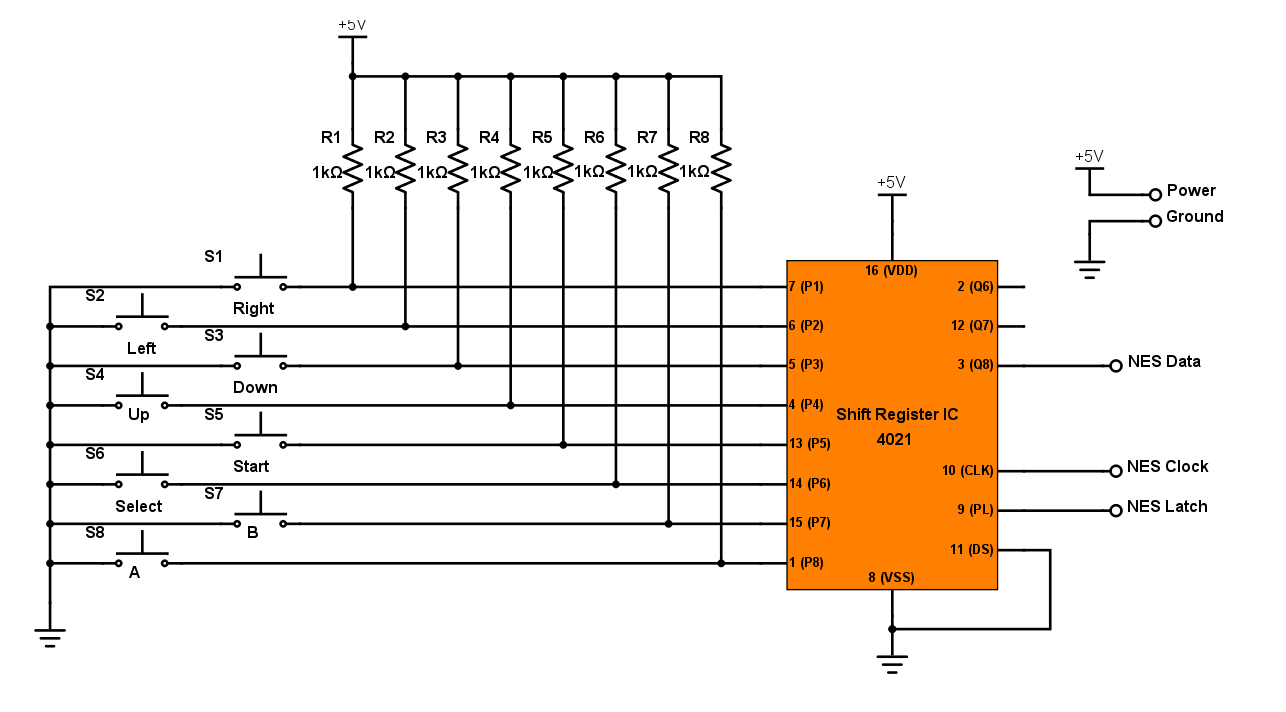
\includegraphics[width=0.8 \linewidth]{images/nesSchema.png}
    \caption{The buttons and shift register inside of an NES controller}
    \label{nesSchematic}
\end{figure}


\begin{figure}[H]
    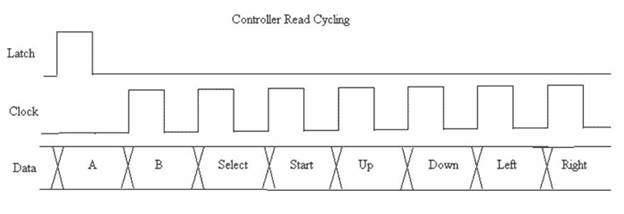
\includegraphics[width=0.8 \linewidth]{images/nesclock.jpg}
    \caption{One shift register worth of data, transmitted after pulsing the latch input high}
    \label{nesClock}
\end{figure}

An example of the NES controller decoder module was provided for us in the course materials, and a discussion of the code is included in the appendix of this document.

\section{HDL Components}

\subsection{Top Module}

INSERT TOP MODULE DIAGRAM HERE

INSERT TOP MODULE DESCRIPTION HERE

\subsection{VGA Output}

INSERT VGA OUTPUT DIAGRAM HERE

Input: The VGA module takes a 50MHz clock signal, a reset signal, and three button signals for the red, green, and blue inputs.

Output: The VGA module outputs a vSync and an hSync signal, and three 4-bit values for the red, green, and blue display colors.

Description: This module is designed to output a 640x480 resolution VGA signal, allowing it to display an RGB color value on a screen. The hSync signal tells a computer monitor how quickly to update each column of the screen, while the vSync signal tells it how quickly to update each row. The color inputs work by having each button press increment a 4-bit counter that goes to the appropriate color output.

\subsubsection{VGA hCounterComp}

INSERT DIAGRAM HERE

Inputs: A 25MHz clock signal, a 50MHz clock signal, and a reset signal.
Outputs: The horizontal sync rate for the VGA output and a signal indicating that it is in the display area for the screen.

Description: The hCounterComp creates the hSync signal for the VGA driver, as well as indicating that the signal is within the display area so that the RGB values can be communicated to the screen. The hSync signal travels through the horizontal row of pixels on the screen, displaying color when appropriate.

\subsubsection{VGA vCounterComp}

INSERT DIAGRAM HERE

Inputs: The hSync signal as a clock, a 50MHz clock signal, and a reset signal.
Outputs: The vertical sync rate for the VGA output and a signal indicating that it is in the display area for the screen.

Description: The vCounterComp module generates the vSync signal for the VGA driver, which tells it when to move on to the next row of pixels, as well as telling it when it is within the displayable area.

\subsubsection{VGA counter}

INSERT DIAGRAM HERE

Inputs: A clock signal and a reset signal.
Outputs: An N-bit binary value.

Description: This counter adds one to its output value each rising clock edge.

\subsubsection{VGA displayMux}

INSERT DIAGRAM HERE

Inputs: A select signal and red, green, and blue binary input values.
Outputs: Either the inputted RGB values or 0 values.

Description: The VGA displayMux decides whether to send the inputted RGB values to the screen or not to, depending on whether or not we are within the displayable area, as given by the hSync and vSync modules.

\subsubsection{VGA comparator}

INSERT DIAGRAM HERE

Inputs: A select signal and red, green, and blue binary input values.
Outputs: Either the inputted RGB values or 0 values.

Description: The VGA displayMux decides whether to send the inputted RGB values to the screen or not to, depending on whether or not we are within the displayable area, as given by the hSync and vSync modules.

\subsubsection{VGA synchronizer}

INSERT DIAGRAM HERE

Inputs: A clock signal and a 1-bit data value.
Outputs: A 1-bit data value.

Description: The synchronizer takes asynchronous inputs and syncs them to the clock edge.

\subsubsection{clockDivBy2}

INSERT DIAGRAM HERE

Inputs: A clock signal and a reset signal.
Outputs: A clock signal half as fast as the input clock signal.

Description: This module takes in a clock input and divides its frequency by 2. For example, a 50MHz clock input would become a 25MHz clock input.

\section{Appendix}

\subsection{Source Code}%%%%%%%%%%%%%%%%%%%%%%%%%%%%%%%%%%%

\subsubsection{NES Controller Reader}
The NES reader module depends on four sub-modules. 
The "Counter4" module is just a resettable four-bit counter.
"NesLatchStateDecoder" receives the count from the "Counter4" counter and outputs a signal when all bits are zero. This signifies the latch signal which corresponds with the first high half of every eight clock cycles.
The "NesClockStateDecoder" module holds the combinational logic which controls the reader module's clock. 
Finally, the "NesDataReceiverDecoder" module reads data from the data wire at the negative edge of the controller's "Clock" signal and outputs a vector of these values. 


\begin{Verbatim}[tabsize = 4]
module NesReader(
  input logic dataYellow,
  input logic clock,
  input logic reset_n,
  output logic latchOrange,
  output logic clockRed,
  output logic up,
  output logic down,
  output logic left,
  output logic right,
  output logic start,
  output logic select,
  output logic a,
  output logic b
  );
  logic [3:0] count;

  Counter4 matt_i1(
    .clk               (clock), 
    .reset_n           (reset_n), 
    .count             (count)
  );

  NesClockStateDecoder matt_i2(
    .controllerState  (count), 
    .nesClock         (clockRed)
  );

  NesLatchStateDecoder matt_i3 (
    .controllerState  (count), 
    .nesLatch         (latchOrange)
  );

  NesDataReceiverDecoder matt_i4 (
    .dataYellow       (dataYellow), 
    .reset_n           (reset_n),
    .controllerState  (count), 
    .readButtons      ({a, b, select, start, up, down, left, right})
  );
endmodule

\begin{Verbatim}
module NesReader(
  input logic dataYellow,
  input logic clock,
  input logic reset_n,
  output logic latchOrange,
  output logic clockRed,
  output logic up,
  output logic down,
  output logic left,
  output logic right,
  output logic start,
  output logic select,
  output logic a,
  output logic b
  );
  logic [3:0] count;

  Counter4 matt_i1(
    .clk               (clock), 
    .reset_n           (reset_n), 
    .count             (count)
  );

  NesClockStateDecoder matt_i2(
    .controllerState  (count), 
    .nesClock         (clockRed)
  );

  NesLatchStateDecoder matt_i3 (
    .controllerState  (count), 
    .nesLatch         (latchOrange)
  );

  NesDataReceiverDecoder matt_i4 (
    .dataYellow       (dataYellow), 
    .reset_n           (reset_n),
    .controllerState  (count), 
    .readButtons      ({a, b, select, start, up, down, left, right})
  );
endmodule


module Counter4(
  input logic clk, reset_n,
  output logic [3:0] count);

  always_ff @ (posedge clk, negedge reset_n)
    if(!reset_n) count <= 4'b0;
    else count <= count + 1;
endmodule


module NesLatchStateDecoder(
  input logic [3:0] controllerState,
  output logic nesLatch);

  always_comb
    case(controllerState)
      4'h0: nesLatch = 1;
      default: nesLatch = 0;
    endcase
endmodule


module NesClockStateDecoder(
  input logic [3:0] controllerState,
  output logic nesClock);

  always_comb
    case (controllerState)
      4'h2: nesClock = 1;
      4'h4: nesClock = 1;
      4'h6: nesClock = 1;
      4'h8: nesClock = 1;
      4'ha: nesClock = 1;
      4'hC: nesClock = 1;
      4'hE: nesClock = 1;
      default: nesClock = 0;
    endcase
endmodule


module Counter4(
  input logic clk, reset_n,
  output logic [3:0] count);

  always_ff @ (posedge clk, negedge reset_n)
    if(!reset_n) count <= 4'b0;
    else count <= count + 1;
endmodule


module NesLatchStateDecoder(
  input logic [3:0] controllerState,
  output logic nesLatch);

  always_comb
    case(controllerState)
      4'h0: nesLatch = 1;
      default: nesLatch = 0;
    endcase
endmodule


module NesClockStateDecoder(
  input logic [3:0] controllerState,
  output logic nesClock);

  always_comb
    case (controllerState)
      4'h2: nesClock = 1;
      4'h4: nesClock = 1;
      4'h6: nesClock = 1;
      4'h8: nesClock = 1;
      4'ha: nesClock = 1;
      4'hC: nesClock = 1;
      4'hE: nesClock = 1;
      default: nesClock = 0;
    endcase
endmodule


module NesDataReceiverDecoder(
  input logic dataYellow,
  input logic reset_n,
  input logic [3:0] controllerState,
  output logic [7:0] readButtons); 

  always_ff @ (posedge controllerState[0], negedge reset_n)
    if(!reset_n) readButtons <= 8'b0;
    else case(controllerState[3:0])
      4'h1: readButtons[7] <= dataYellow;	//a button
      4'h3: readButtons[6] <= dataYellow;	//b button
      4'h5: readButtons[5] <= dataYellow;	//select button
      4'h7: readButtons[4] <= dataYellow;	//start button
      4'h9: readButtons[3] <= dataYellow;	//up button
      4'hB: readButtons[2] <= dataYellow;	//down button
      4'hD: readButtons[1] <= dataYellow;	//left button
      4'hF: readButtons[0] <= dataYellow;	//right button
      default: readButtons <= readButtons;
    endcase
endmodule
\end{Verbatim}

\subsubsection{Square Wave Generator}

\begin{Verbatim}[tabsize=4]
module periodTime(input logic clk,
					input logic [2:0] data,
					output logic q);
					
int compareNumber;
int count;

always_comb
		case(data)
			0: compareNumber = 6400;	// just mod input clock until audio spectrum periods
			1: compareNumber = 3200;	// one octave
			2: compareNumber = 1600;
			3: compareNumber = 8000;
			
			4: compareNumber = 4000;
			5: compareNumber = 2000;
			6: compareNumber = 1000;
			7: compareNumber = 500;		// consider adding default case
		endcase
			
always_ff @(posedge clk)
	begin
		if (count >= compareNumber)	// could modify to not restart notes when changed
			count <= 0;
		else 
			count <= count +1;
	end

always_comb
	begin
			if( count < compareNumber)				
				q = (count > compareNumber/2); 	//assigns output with initial low
			else 
				q = 0;
	end

endmodule
\end{Verbatim}

\subsubsection{VGA Output}

\begin{Verbatim}
module vgaOutput
		(input clock50MHz,
		 input inReset,
		 input inRed,
		 input inGreen,
		 input inBlue,
		 output hSync,
		 output vSync,
		 output [3:0] outRed, outGreen, outBlue);
	
	vga_counter #(.N(4)) redCounter (
		.clk(inRed),
		.reset(inReset),
		.q(redCount)
	);
	
	vga_counter #(.N(4)) greenCounter (
		.clk(inGreen),
		.reset(inReset),
		.q(greenCount)
	);
	
	vga_counter #(.N(4)) blueCounter (
		.clk(inBlue),
		.reset(inReset),
		.q(blueCount)
	);

	clockDivBy2 clockDivider(
		.clock50MHz(clock50MHz),
		.inReset(~inReset),
		.outClock(clock25MHz)
	);
	
	vga_hCounterComp #(.a(10'd96), .b(10'd48), .c(10'd640), .d(10'd16)) hSyncCounter (
		.inClock(clock25MHz),
		.clock50MHz(clock50MHz),
		.inReset(~inReset),
		.signal(hSync),
		.displaySignal(hSignal)
	);
	
	clockDivBy2 syncDivider(
		.clock50MHz(hSync),
		.inReset(~inReset),
		.outClock(hClock)
	); 
	
	vga_vCounterComp #(.a(10'd2), .b(10'd33), .c(10'd480), .d(10'd10)) vSyncCounter (
		.inClock(hClock),
		.clock50MHz(clock50MHz),
		.inReset(~inReset),
		.signal(vSync),
		.displaySignal(vSignal)
	);
	
	vga_displayMux display (
		.select(hSignal & vSignal),
		.inRed(redCount),
		.inGreen(greenCount),
		.inBlue(blueCount),
		.outRed(outRed),
		.outGreen(outGreen),
		.outBlue(outBlue)
	);

endmodule
\end{Verbatim}

\subsubsection{VGA hCounterComp}

\begin{Verbatim}
module vga_hCounterComp #(parameter a = 10, b = 10, c = 10, d = 10)
		(input inClock,
		 input clock50MHz,
		 input inReset,
		 output signal,
		 output displaySignal);
		 
	logic [9:0] currentCount;

	vga_counter #(.N(10)) count1 (
		.clk(inClock),
		.reset(cntReset | inReset),
		.q(currentCount)
	);
	
	vga_comparator #(.N(10)) aTob (
		.a(currentCount),
		.b(a),
		.gte(signal)
	);
	
	vga_comparator #(.N(10)) bToc (
		.a(currentCount),
		.b(a + b),
		.gte(disp1)
	);
	
	vga_comparator #(.N(10)) cToD (
		.a(currentCount),
		.b(a + b + c),
		.lt(disp2)
	);
	
	vga_comparator #(.N(10)) reset (
		.a(currentCount),
		.b(a + b + c + d),
		.eq(compSignal)
	);
	
	vga_synchronizer sync1 (
		.clk(clock50MHz),
		.d(compSignal),
		.q(cntReset)
	);
	
	assign displaySignal = disp1 & disp2;

endmodule
\end{Verbatim}

\subsubsection{VGA vCounterComp}

\begin{Verbatim}
module vga_vCounterComp #(parameter a = 10, b = 10, c = 10, d = 10)
		(input inClock,
		 input clock50MHz,
		 input inReset,
		 output signal,
		 output displaySignal);
		 
	logic [9:0] currentCount;

	vga_counter #(.N(10)) count1 (
		.clk(inClock),
		.reset(cntReset | inReset),
		.q(currentCount)
	);
	
	vga_comparator #(.N(10)) aTob (
		.a(currentCount),
		.b(a),
		.gte(signal)
	);
	
	vga_comparator #(.N(10)) bToc (
		.a(currentCount),
		.b(a + b),
		.gte(disp1)
	);
	
	vga_comparator #(.N(10)) cToD (
		.a(currentCount),
		.b(a + b + c),
		.lt(disp2)
	);
	
	vga_comparator #(.N(10)) reset (
		.a(currentCount),
		.b(a + b + c + d),
		.eq(compSignal)
	);
	
	vga_synchronizer sync1 (
		.clk(clock50MHz),
		.d(compSignal),
		.q(cntReset)
	);
	
	assign displaySignal = disp1 & disp2;

endmodule
\end{Verbatim}

\subsubsection{VGA counter}

\begin{Verbatim}
module vga_counter #(parameter N = 4)
		(input logic clk,
		 input logic reset,
		 output logic [N-1:0] q);

	always_ff @(posedge clk, posedge reset) begin
		if (reset)	q <= 0;
		else			q <= q + 1;
	end

endmodule
\end{Verbatim}

\subsubsection{VGA displayMux}

\begin{Verbatim}
module vga_counter #(parameter N = 4)
		(input logic clk,
		 input logic reset,
		 output logic [N-1:0] q);

	always_ff @(posedge clk, posedge reset) begin
		if (reset)	q <= 0;
		else			q <= q + 1;
	end

endmodule
\end{Verbatim}

\subsubsection{VGA comparator}

\begin{Verbatim}
module vga_comparator #(parameter N = 1)
		(input logic [N-1:0] a, b,
		 output logic eq, neq, lt, lte, gt, gte);

	assign eq	= (a == b);
	assign neq	= (a != b);
	assign lt	= (a < b);
	assign lte	= (a <= b);
	assign gt	= (a > b);
	assign gte	= (a >= b);

endmodule
\end{Verbatim}

\subsubsection{VGA synchronizer}

\begin{Verbatim}
module vga_synchronizer
		(input logic clk,
		 input logic d,
		 output logic q);

	logic n1;
	
	always_ff @(posedge clk)
		begin
			n1 <= d;
			q <= n1;
		end

endmodule
\end{Verbatim}

\subsubsection{clockDivBy2}

\begin{Verbatim}
module clockDivBy2
	(input clock50MHz,
	 input inReset,
	 output reg outClock);

	always @(posedge clock50MHz) begin
		if (inReset)
			  outClock <= 1'b0;
		else
			  outClock <= ~outClock;
	end

endmodule
\end{Verbatim}

\subsection{Simulation Results}%%%%%%%%%%%%%%%%%%%%%%%%%%%%%

\subsubsection{NES Controller Reader}
\begin{figure}[H]
    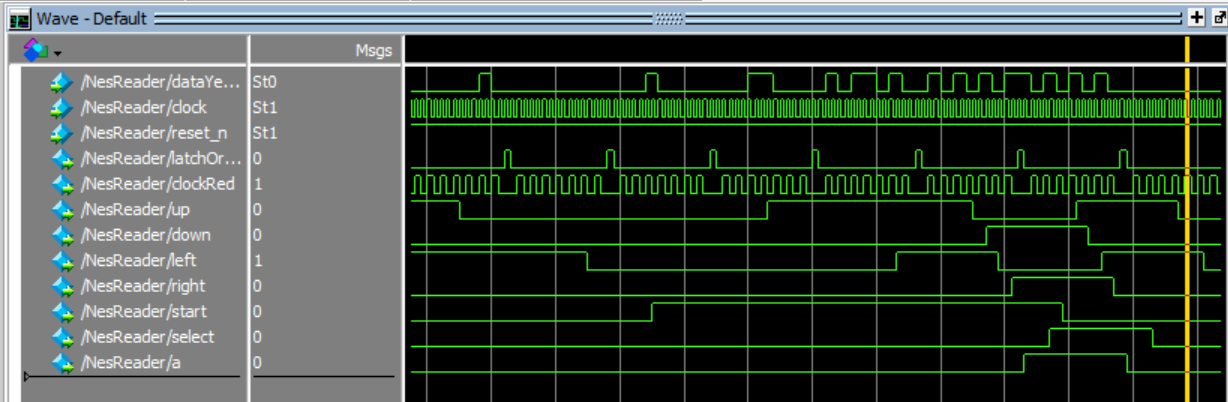
\includegraphics[width=0.8 \linewidth]{images/NESSIM.png}
    \caption{"Button Mashing" on the NES}
    \label{nesButtonMash}
\end{figure}

At first, I wanted to test the NES controller reader by just simulating a bunch of random inputs as seen in Figure \ref{nesButtonMash}. I remembered the NES game CONTRA had a cheat code that involved most of the controller's buttons (all but SELECT). The "Contra Code" was then simulated with the following ModelSim macro code.
 
\begin{figure}[H]
    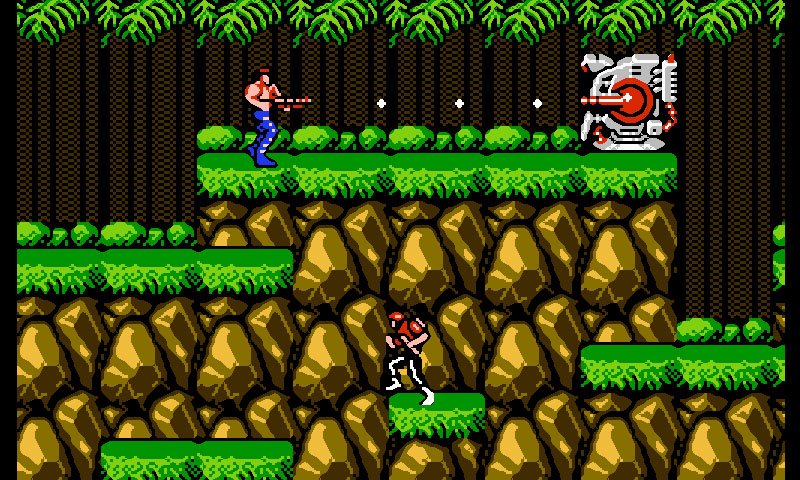
\includegraphics[width=0.8 \linewidth]{images/contra.jpg}
    \caption{CONTRA screenshot}
    \label{contra}
\end{figure}

\begin{figure}[H]
    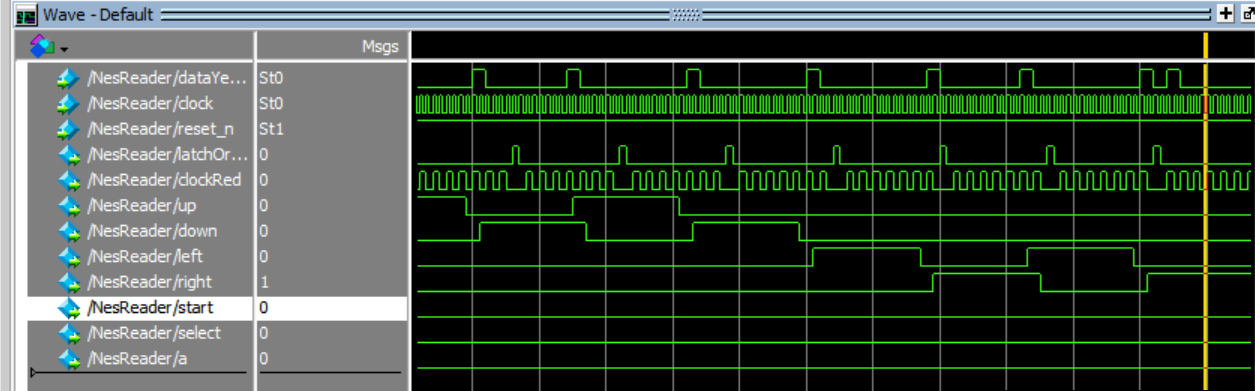
\includegraphics[width=0.8 \linewidth]{images/NESSIMcontra.png}
    \caption{Simulating the "Contra Code" }
    \label{contraSim}
\end{figure}

\begin{verbatim}

force -freeze sim:/NesReader/dataYellow 0 0, 0 {20 ps} , 0 {40 ps} , 0 {60 ps} , 
    1 {80 ps} , 0 {100 ps} , 0 {120 ps} , 0 {140 ps}	#up
force -freeze sim:/NesReader/dataYellow 0 0, 0 {20 ps} , 0 {40 ps} , 0 {60 ps} , 
    0 {80 ps} , 1 {100 ps} , 0 {120 ps} , 0 {140 ps}	#down
force -freeze sim:/NesReader/dataYellow 0 0, 0 {20 ps} , 0 {40 ps} , 0 {60 ps} , 
    1 {80 ps} , 0 {100 ps} , 0 {120 ps} , 0 {140 ps}	#up
force -freeze sim:/NesReader/dataYellow 0 0, 0 {20 ps} , 0 {40 ps} , 0 {60 ps} , 
    0 {80 ps} , 1 {100 ps} , 0 {120 ps} , 0 {140 ps}	#down
force -freeze sim:/NesReader/dataYellow 0 0, 0 {20 ps} , 0 {40 ps} , 0 {60 ps} , 
    0 {80 ps} , 0 {100 ps} , 1 {120 ps} , 0 {140 ps}	#left
force -freeze sim:/NesReader/dataYellow 0 0, 0 {20 ps} , 0 {40 ps} , 0 {60 ps} , 
    0 {80 ps} , 0 {100 ps} , 0 {120 ps} , 1 {140 ps}	#right
force -freeze sim:/NesReader/dataYellow 0 0, 0 {20 ps} , 0 {40 ps} , 0 {60 ps} , 
    0 {80 ps} , 0 {100 ps} , 1 {120 ps} , 0 {140 ps}	#left
force -freeze sim:/NesReader/dataYellow 0 0, 0 {20 ps} , 0 {40 ps} , 0 {60 ps} , 
    0 {80 ps} , 0 {100 ps} , 0 {120 ps} , 1 {140 ps}	#right
force -freeze sim:/NesReader/dataYellow 0 0, 1 {20 ps} , 0 {40 ps} , 0 {60 ps} , 
    0 {80 ps} , 0 {100 ps} , 0 {120 ps} , 0 {140 ps}	#b	
force -freeze sim:/NesReader/dataYellow 1 0, 0 {20 ps} , 0 {40 ps} , 0 {60 ps} , 
    0 {80 ps} , 0 {100 ps} , 0 {120 ps} , 0 {140 ps}	#a
force -freeze sim:/NesReader/dataYellow 0 0, 0 {20 ps} , 0 {40 ps} , 1 {60 ps} , 
    0 {80 ps} , 0 {100 ps} , 0 {120 ps} , 0 {140 ps}	start
\end{verbatim}

\subsubsection{Square Wave Generator}

Our square wave generator module works by receiving a 3-bit data bus and outputs successive octaves of a music note. This module was simply tested by simulating various data inputs on the 3-bit bus. This is pictured in figure \ref{squareSim}.

\begin{figure}[H]
    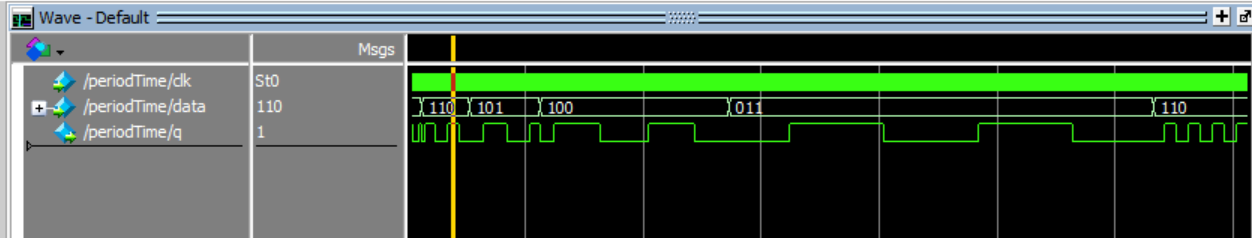
\includegraphics[width=0.8 \linewidth]{images/squareSim.png}
    \caption{Simulating button inputs to control the square wave oscillator}
    \label{squareSim}
\end{figure}

\subsubsection{VGA Output}

\begin{figure}[H]
    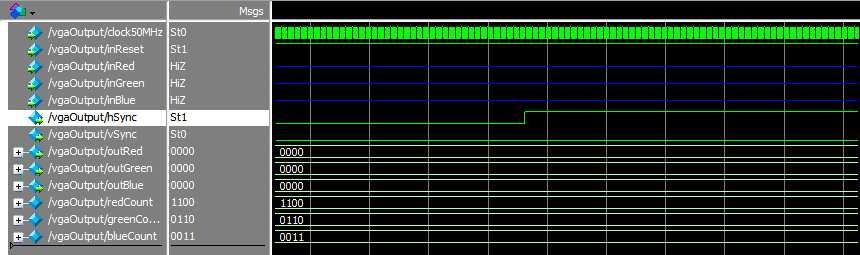
\includegraphics[width=0.8 \linewidth]{images/vgaOutputSim.png}
    \caption{Simulating inputs to the VGA output}
    \label{vgaOutputSim}
\end{figure}

Do File:

\begin{Verbatim}
add wave clock50MHz
add wave inReset
add wave inRed
add wave inGreen
add wave inBlue
add wave hSync
add wave vSync
add wave outRed
add wave outGreen
add wave outBlue
add wave redCount
add wave greenCount
add wave blueCount
force -drive clock50MHz -r 4 0 0, 1 2
force -deposit inReset 0
run
force -deposit inReset 1
run
force -deposit redCount 4'b1100
force -deposit greenCount 4'b0110
force -deposit blueCount 4'b0011
run
\end{Verbatim}

\subsubsection{VGA hCounterComp}

\begin{figure}[H]
    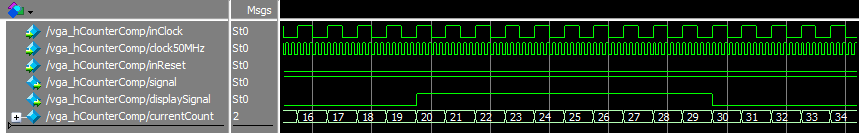
\includegraphics[width=0.8 \linewidth]{images/vgaHCounterCompSim.png}
    \caption{Simulating inputs to the VGA hCounterComp. For this simulation, the range from 20 to 30 is the display range}
    \label{vgaHCounterCompSim}
\end{figure}

Do File:

\begin{Verbatim}
add wave inClock
add wave clock50MHz
add wave inReset
add wave signal
add wave displaySignal
add wave currentCount
force -drive inClock -r 50 0 0, 1 25
force -drive clock50MHz -r 10 0 0, 1 5
force -deposit inReset 1
run
force -deposit inReset 0
run
\end{Verbatim}

\subsubsection{VGA vCounterComp}

\begin{figure}[H]
    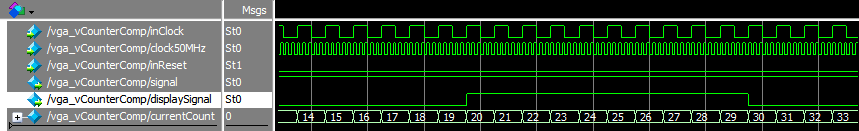
\includegraphics[width=0.8 \linewidth]{images/vgaVCounterCompSim.png}
    \caption{Simulating inputs to the VGA vCounterComp. For this simulation, the range from 20 to 30 is the display range}
    \label{vgaVCounterCompSim}
\end{figure}

Do File:

\begin{Verbatim}
add wave inClock
add wave clock50MHz
add wave inReset
add wave signal
add wave displaySignal
add wave currentCount
force -drive inClock -r 50 0 0, 1 25
force -drive clock50MHz -r 10 0 0, 1 5
force -deposit inReset 1
run
force -deposit inReset 0
run
\end{Verbatim}

\subsubsection{VGA counter}

\begin{figure}[H]
    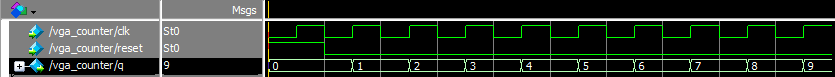
\includegraphics[width=0.8 \linewidth]{images/vgaCounterSim.png}
    \caption{Simulating inputs to the VGA counter}
    \label{vgaCounterSim}
\end{figure}

Do File:

\begin{Verbatim}
add wave clk
add wave reset
add wave q
force -drive clk -r 100 0 0, 1 50
force -deposit reset 1
run
force -deposit reset 0
run
\end{Verbatim}

\subsubsection{VGA displayMux}

\begin{figure}[H]
    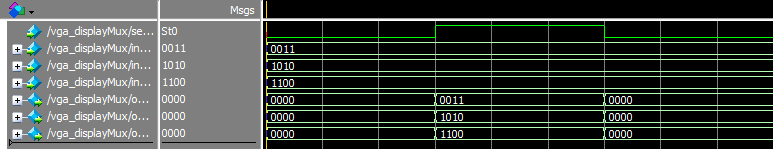
\includegraphics[width=0.8 \linewidth]{images/vgaDisplayMuxSim.png}
    \caption{Simulating inputs to the VGA displayMux}
    \label{vgaDisplayMuxSim}
\end{figure}

Do File:

\begin{Verbatim}
add wave select
add wave inRed
add wave inGreen
add wave inBlue
add wave outRed
add wave outGreen
add wave outBlue
force -deposit inRed 4'b0011
force -deposit inGreen 4'b1010
force -deposit inBlue 4'b1100
force -deposit select 0
run
force -deposit select 1
run
force -deposit select 0
run
\end{Verbatim}

\subsubsection{VGA comparator}

\begin{figure}[H]
    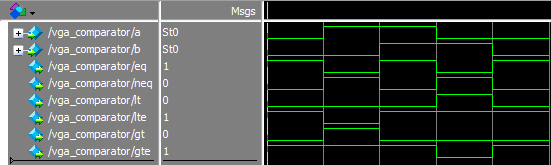
\includegraphics[width=0.8 \linewidth]{images/vgaCompSim.png}
    \caption{Simulating inputs to the VGA comparator}
    \label{vgaCompSim}
\end{figure}

Do file:

\begin{Verbatim}
add wave a
add wave b
add wave eq
add wave neq
add wave gt
add wave gte
add wave lt
add wave lte

force -deposit a 0
force -deposit b 0
run
force -deposit a 1
run
force -deposit b 1
run
force -deposit a 0
run
force -deposit b 0
run
\end{Verbatim}

\subsubsection{VGA synchronizer}

\begin{figure}[H]
    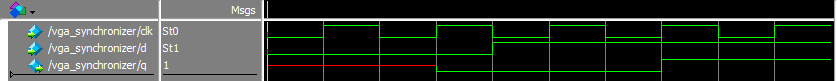
\includegraphics[width=0.8 \linewidth]{images/vgaSyncSim.png}
    \caption{Simulating inputs to the VGA synchronizer module}
    \label{vgaSyncSim}
\end{figure}

Do File:

\begin{Verbatim}
add wave clk
add wave d
add wave q
force -drive clk -r 200 0 0, 1 100
force -deposit d 0
run
force -deposit d 1
run
\end{Verbatim}

\subsubsection{clockDivBy2}

\begin{figure}[H]
    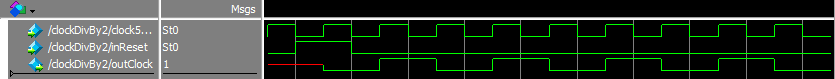
\includegraphics[width=0.8 \linewidth]{images/clockDivBy2Sim.png}
    \caption{Simulating inputs to the clockDivBy2 module}
    \label{clockDivBy2Sim}
\end{figure}

Do File:

\begin{Verbatim}
add wave clock50MHz
add wave inReset
add wave outClock
force -drive clock50MHz -r 100 0 0, 1 50
force -deposit inReset 0
run
force -deposit inReset 1
run
force -deposit inReset 0
run
\end{Verbatim}

%\includepdf[page=-]{Ch3Example}

\end{document}
